\documentclass[12pt, a4paper, addpoints]{exam}
\usepackage{amsmath}
\usepackage{pgfmath}
\usepackage{xcolor}
\usepackage{multicol} % For multi-column layout
\usepackage{mdframed} % For framed boxes
\usepackage{tikz} % For drawing and diagrams

% Load the expandcubic command from expandcubic.tex if needed
% 
\documentclass[12pt, a4paper, addpoints]{exam}

\title{Synthetic Division}


\pagestyle{empty} % Suppress page numbers
\usepackage[top=5mm, bottom=20mm, left=11mm, right=11mm]{geometry}
\usepackage{amsmath} 
\usepackage{multicol} 
\usepackage{tabularx}
\usepackage{pgfmath}
\usepackage{xcolor} 
\pagestyle{empty}
% \author{Mr Downes}
\newcommand{\ts}{\vspace{16mm}}
\newcommand{\ms}{\vspace{20mm}}
\newcommand{\bs}{\vspace{30mm}}
\newcommand{\ls}{\vspace{30mm}}
\newcommand{\hs}{\vspace{30mm}}
\usepackage{array}     % For centering text vertically
\usepackage{graphicx}  % For rotating text

\date{}



% Define the cubic expansion
\newcommand{\expandquadratic}[5]{
    \pgfmathsetmacro{\termone}{int(#1*#4)} % Coefficient of x^3
    \pgfmathsetmacro{\termtwo}{int(#1*#5 + #2*#4)} % Coefficient of x^2
    \pgfmathsetmacro{\termthree}{int(#2*#5 + #3*#4)} % Coefficient of x
    \pgfmathsetmacro{\termfour}{int(#3*#5)} % Constant term
    
    \ifnum\termone=0\else
        \ifnum\termone=1 x^3\else
        \ifnum\termone=-1 -x^3\else \termone x^3\fi\fi
    \fi
    \ifnum\termtwo=0\else
        \ifnum\termtwo>0 
            \ifnum\termtwo=1 + x^2\else + \termtwo x^2\fi
        \else
            \ifnum\termtwo=-1 - x^2\else \termtwo x^2\fi
        \fi
    \fi
    \ifnum\termthree=0\else
        \ifnum\termthree>0 
            \ifnum\termthree=1 + x\else + \termthree x\fi
        \else
            \ifnum\termthree=-1 - x\else \termthree x\fi
        \fi
    \fi
    \ifnum\termfour=0\else
        \ifnum\termfour>0 + \termfour\else \termfour\fi
    \fi
}

% Define synthetic division
\newcommand{\syntheticdiv}[5]{
    \dfrac{
        % Call the expandquadratic to generate the cubic expression
        \expandquadratic{#1}{#2}{#3}{#4}{#5}
    }{
        % Denominator (linear factor)
        \ifnum#4=1
            x \pm #5
        \else
            #4x \pm #5
        \fi
    }
}


\begin{document}
% Adjust vertical spacing before and after the title

\maketitle
\vspace{-28mm}
% \section{Calculations using powers  $a^p$  and $a^q$ }
 % \huge

\large

\begin{questions}



% \question Recall and  understanding these indices and logarithms identities from page 21.
% \Large
% % \begin{multicols}{2}
% \begin{parts}
% \part \text{Product of Powers — Add the exponents} \hfill $a^p a^q = a^{p+q}$

% \part \text{Quotient of Powers — Subtract  the exponents} \hfill $\dfrac{a^p}{a^q} = a^{p-q}$
% \part \text{Power of a Power — Multiply the exponents} \hfill $(a^p)^q = a^{pq}$

% \part \text{Zero Exponent — Any non-zero base raised to zero equals 1:} \hfill $a^0 = 1$

% \part \text{Negative Exponent — Recipricate  and change the sign} \hfill $a^{-p} = \dfrac{1}{a^p}$


% % \part \text{Power of a Quotient} \hfill $\left( \dfrac{a}{b} \right)^p = \frac{a^p}{b^p}$

% \part \text{Power of a Product — Distribute the exponent} \hfill $(ab)^p = a^p b^p$


% \end{parts}
% % \end{multicols}

\large

\question Apply the Product of Powers rule — Add the exponents to simplify.

\setlength{\columnsep}{20pt}
\begin{multicols}{2}
\begin{parts}
\part \syntheticdiv{2}{3}{4}{1}{5}
\part \expandquadratic{1}{6}{-17}{2}{5}
\part \expandquadratic{1}{-10}{-3}{1}{7}
\end{parts}
\end{multicols}
\ts





\end{questions}


\end{document}


% Define the new elimination solution command (if relevant for this document)
% Here you'd add any other custom commands you need.

\begin{document}

\title{Mathematics Exam}
\author{Your Name}
\date{\today}
\maketitle

\section*{Instructions}
Answer all questions. Show all work for full credit.

\begin{questions}

% Question 1: Simple math question
\question Find the x- and y-intercepts of the following line:
\[
3x + 2y = 6
\]

% Question 2: Example using multicols and parts
\question Expand the following expression and divide it by the binomial.

\begin{multicols}{2}
    \begin{parts}
        \part \( (2x^2 + 3x + 5)(x - 2) \)
        \part \( (4x^2 - 2x + 7)(x + 3) \)
    \end{parts}
\end{multicols}

% Question 3: A diagram using TikZ
\question Sketch the graph of the following quadratic equation using TikZ.
\[
y = x^2 - 4x + 3
\]

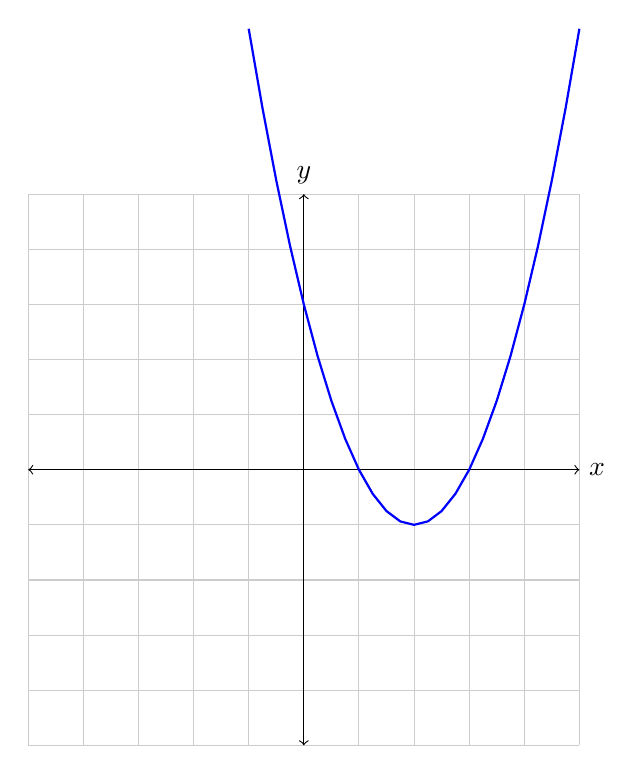
\begin{tikzpicture}[scale=0.7]
    \draw[thin, gray!40] (-5,-5) grid (5,5);
    \draw[<->] (-5,0) -- (5,0) node[right] {$x$};
    \draw[<->] (0,-5) -- (0,5) node[above] {$y$};
    \draw[thick,blue] plot[domain=-1:5] (\x,{(\x)^2 - 4*(\x) + 3});
\end{tikzpicture}

\end{questions}

\end{document}
